\documentclass[aspectratio=169]{beamer}
\usetheme{Madrid}

\usepackage{amsmath}
\usepackage{amssymb}
\usepackage{booktabs}
\usepackage{graphicx}
\usepackage[strings]{underscore}

\title{\texttt{s\_lolrECB}: ECB Intervention and Simulation Results}
\author{}
\date{\today}

\begin{document}

\begin{frame}
    \titlepage
\end{frame}

\begin{frame}{ECB Model: Sovereign Problem}
\footnotesize
\[
V^{ND}(b,g,s,\varepsilon)=
\max_{b'}
\left\{
u(c^{ND})+\beta g^{1-\gamma}
\mathbb{E}\!\left[
\max\{V^{ND}(b',g',s',\varepsilon'),V^D(b',g',s',\varepsilon')\}
\mid g,s\right]
\right\}
\]
\[
c^{ND}=y(g,\varepsilon)-b+n(b',g,s),
\qquad
y(g,\varepsilon)=g e^{\sigma_\varepsilon\varepsilon},
\qquad
n(b',g,s)=\frac{g b'}{R(b',g,s)}
\]
\[
\begin{aligned}
V^D(b,g,s,\varepsilon)
={}&u\!\left(\phi_g y(g,\varepsilon)\right)+\beta g^{1-\gamma}
\mathbb{E}\!\left[
\theta V^D\!\left(\frac{b}{g},g',s',\varepsilon'\right)\right.\\[-1mm]
&\left.\quad +(1-\theta)
\max\!\left\{
V^{ND}\!\left(\kappa\frac{b}{g},g',s',\varepsilon'\right),
V^D\!\left(\frac{b}{g},g',s',\varepsilon'\right)
\right\}
\middle| g,s
\right].
\end{aligned}
\]

\medskip
\begin{block}{Key Difference From Direct LOLR Lending}
There is no sovereign debt state $\ell$: the ECB buys private bonds after market clearing rather
than lending directly to the sovereign.
\end{block}
\end{frame}

\begin{frame}{ECB Facility and the Private-Bond Schedule}
\small
\[
Q(b,g,s,\varepsilon)=(1-d)+dX,
\qquad
H(b',g,s)=\frac{\mathbb{E}[Q(b',g',s',\varepsilon')\mid g,s]}{1+r^\ast}
\]
\[
P(g,s)=
\begin{cases}
\dfrac{1}{1+r^\ast+\sigma^\ell}, & \text{repayment, }g=g_L,\ s=s_b,\\[5pt]
0, & \text{otherwise,}
\end{cases}
\qquad
L(b',g,s)=\pi P(g,s)+(1-\pi)H(b',g,s)
\]
\[
R(b',g,s)=\frac{1}{\max\{H(b',g,s),L(b',g,s)\}},
\qquad
n(b',g,s)=\frac{g b'}{R(b',g,s)}
\]

\begin{columns}[T,onlytextwidth]
\column{0.54\textwidth}
\begin{block}{Intervention}
Only lenders holding bonds issued in repayment, low growth, and the bad sunspot
may use the facility. They queue only if $L>H$.
\end{block}
\column{0.43\textwidth}
\begin{block}{Reported Policy Grid}
\[
\begin{aligned}
\pi&\in\{0,.25,.50,.75,1\},\\
\sigma^\ell&\in\{.04,.06,.08,.10\}.
\end{aligned}
\]
Baseline: $\pi=.50$, $\sigma^\ell=.04$.
\end{block}
\end{columns}
\end{frame}

\begin{frame}{Baseline Policy: Private Schedule and Issuance}
\begin{columns}[T,onlytextwidth]
\column{0.50\textwidth}
\centering
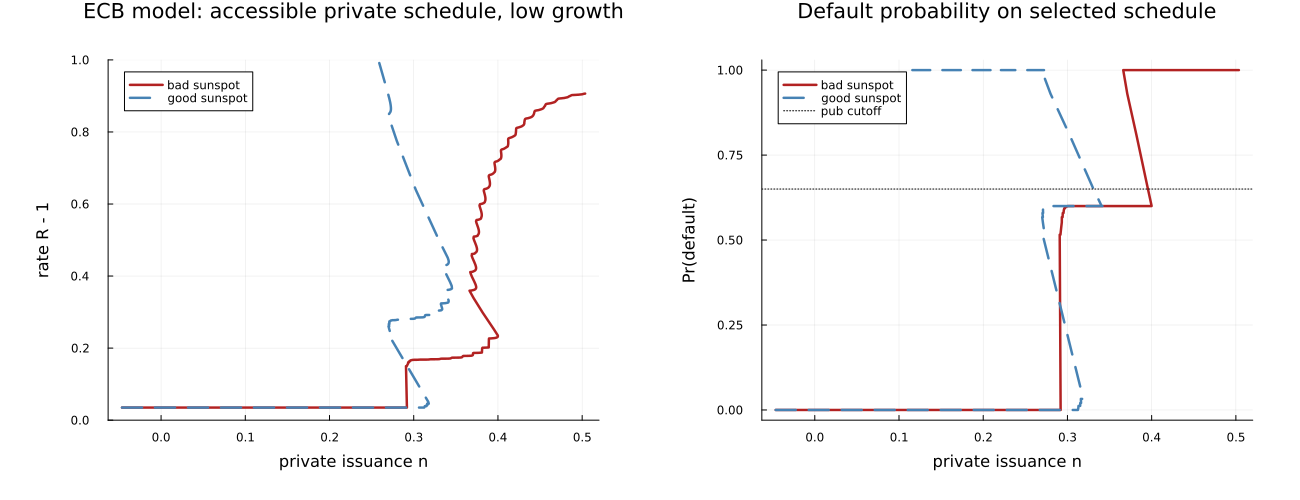
\includegraphics[width=\linewidth]{../../1period_s_lolrECB/result/figures/ecb_selected_schedule.png}

{\scriptsize Selected private schedule in low growth}

\column{0.50\textwidth}
\centering
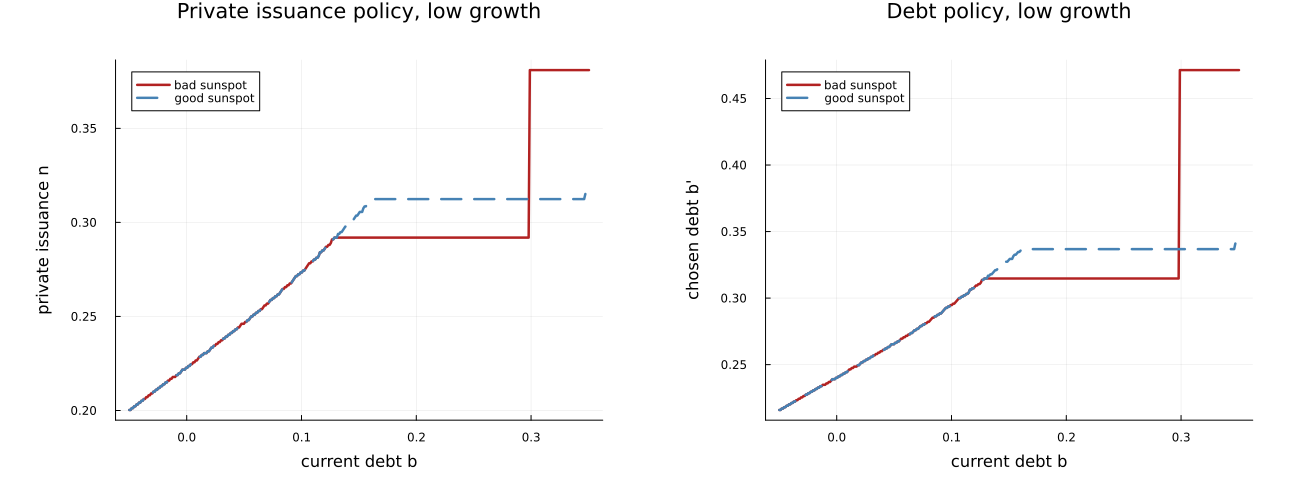
\includegraphics[width=\linewidth]{../../1period_s_lolrECB/result/figures/ecb_private_policy.png}

{\scriptsize Equilibrium private borrowing policy}
\end{columns}
\end{frame}

\begin{frame}{Baseline Policy: ECB Facility and Default}
\begin{columns}[T,onlytextwidth]
\column{0.50\textwidth}
\centering
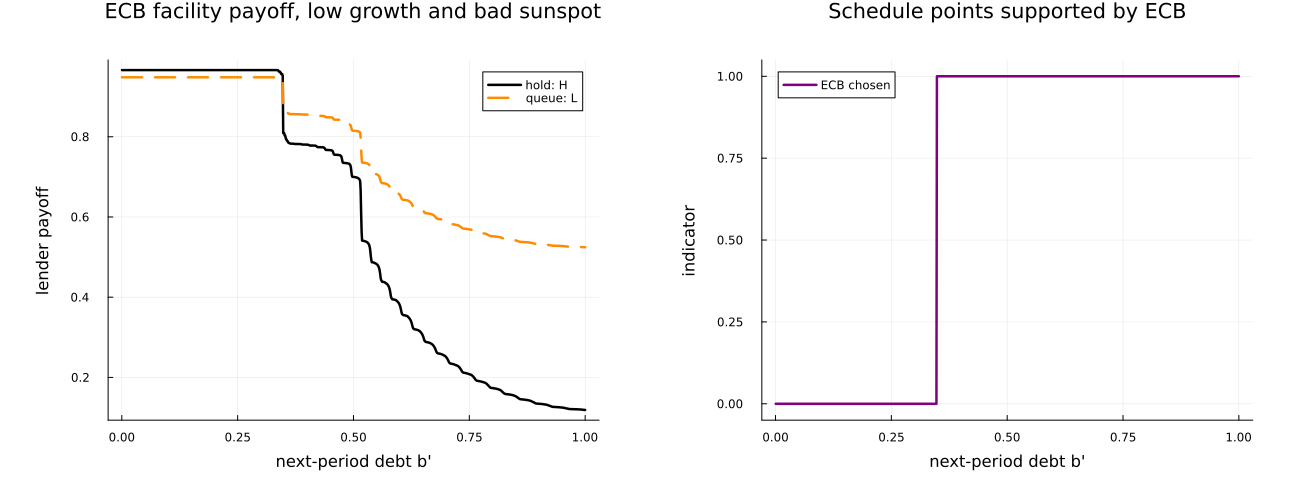
\includegraphics[width=\linewidth]{../../1period_s_lolrECB/result/figures/ecb_facility_payoff.png}

{\scriptsize Hold-versus-facility payoff comparison}

\column{0.50\textwidth}
\centering
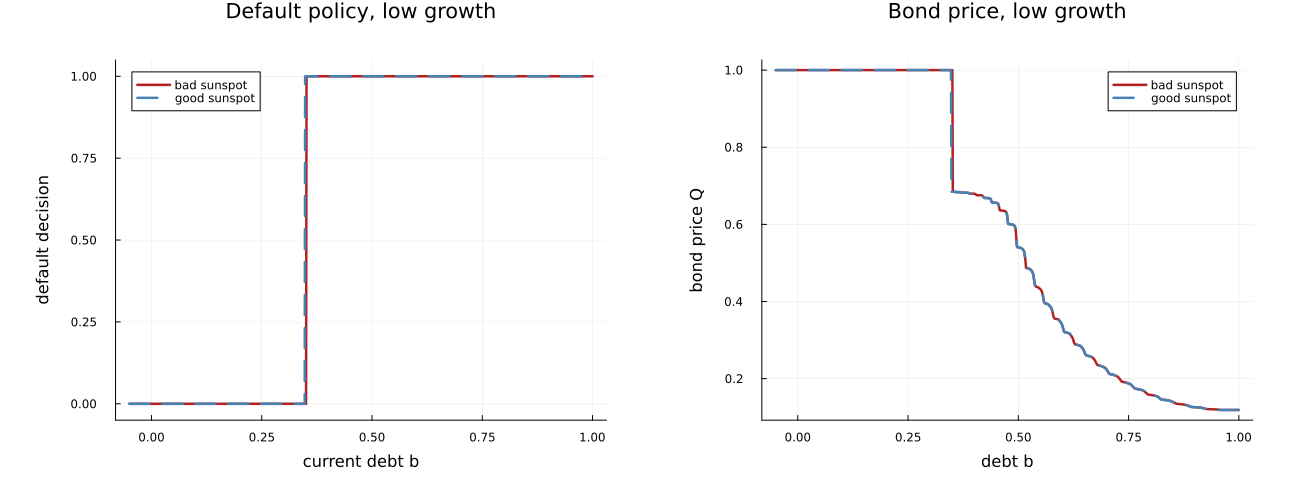
\includegraphics[width=\linewidth]{../../1period_s_lolrECB/result/figures/ecb_default_and_price.png}

{\scriptsize Default policy and bond price}
\end{columns}
\end{frame}

\begin{frame}{Baseline Simulation: Issuance and ECB Support}
\begin{columns}[T,onlytextwidth]
\column{0.50\textwidth}
\centering
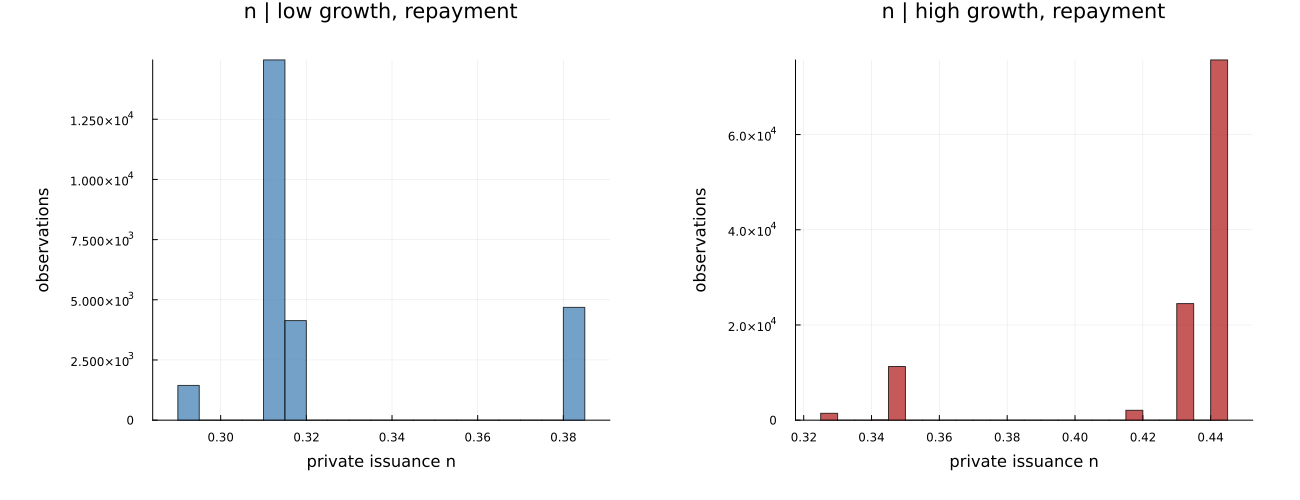
\includegraphics[width=\linewidth]{../../1period_s_lolrECB/result/figures/ecb_issuance_distribution.png}

{\scriptsize Simulated distribution of private issuance}

\column{0.50\textwidth}
\centering
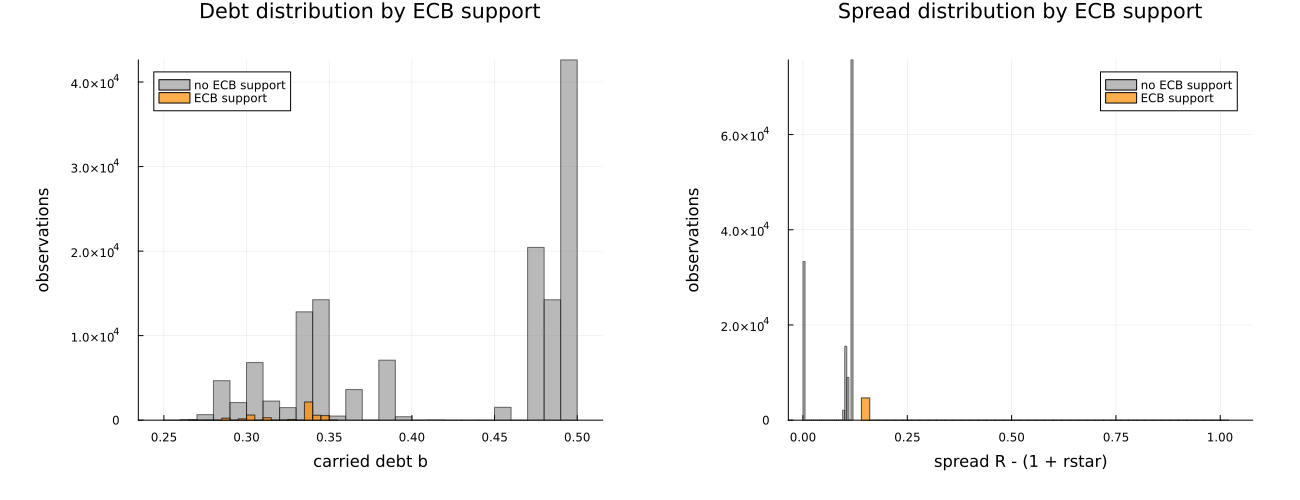
\includegraphics[width=\linewidth]{../../1period_s_lolrECB/result/figures/ecb_support_distributions.png}

{\scriptsize Outcomes with and without ECB support}
\end{columns}
\end{frame}

\begin{frame}{Baseline Simulation: Growth-Transition Outcomes}
\centering
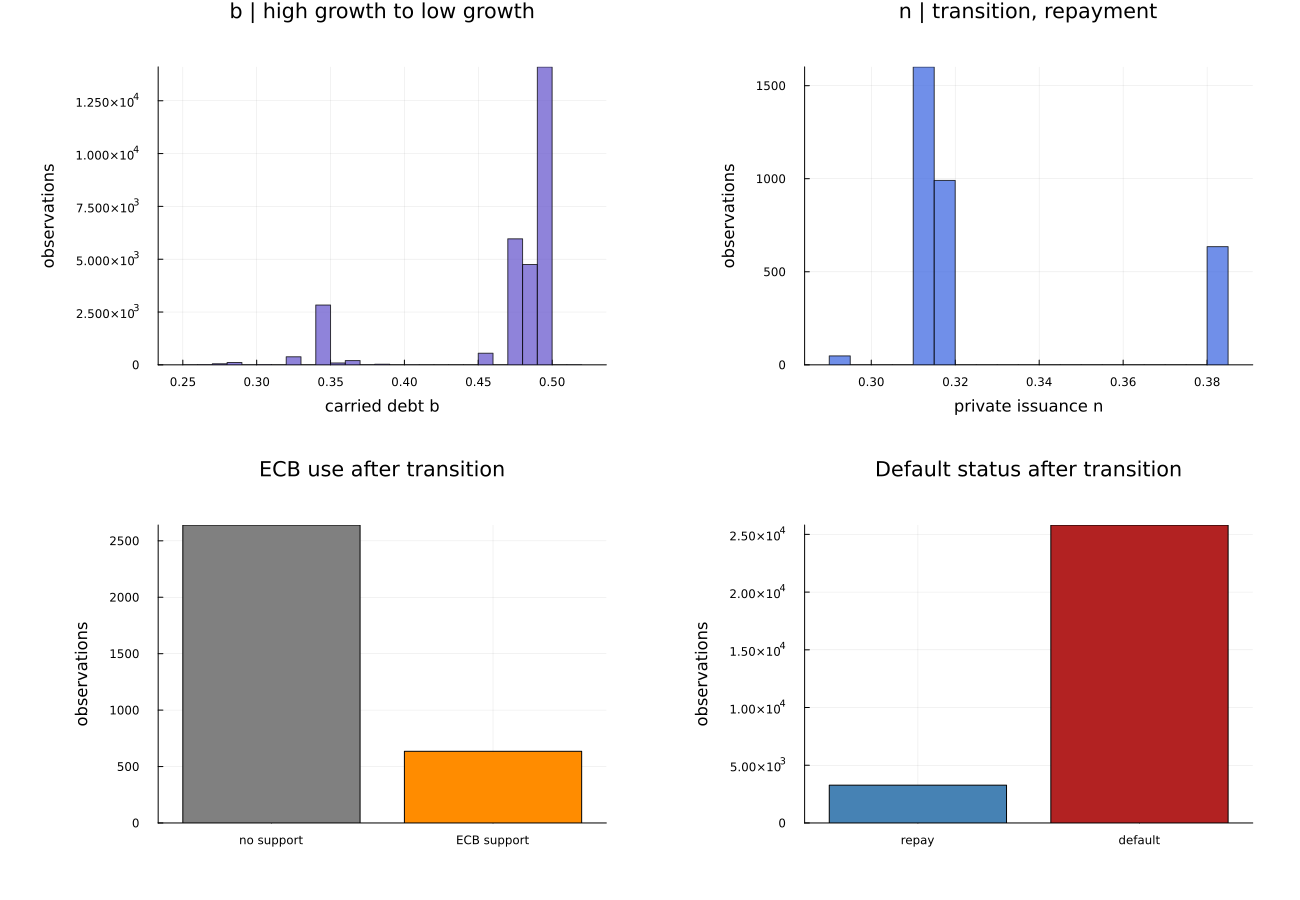
\includegraphics[height=0.77\textheight]{../../1period_s_lolrECB/result/figures/ecb_transition_distributions.png}

{\scriptsize Simulated outcomes around $g_H \rightarrow g_L$ transitions}
\end{frame}


\begin{frame}[shrink=18]{Baseline Table}
\hypertarget{main-sim-table}{}
\scriptsize
\centering
\begingroup
\setlength{\tabcolsep}{4pt}
\renewcommand{\arraystretch}{0.92}
\begin{table}[!htbp]
\centering
\caption{ECB baseline simulated moments}
\begin{tabular}{lc}
\toprule
Moment & $\pi=50\%,\ \sigma^\ell=4\%$ \\
\midrule
\multicolumn{2}{l}{\textit{First moments}} \\
avg(spread) & 0.0879 \\
avg(qb/y) & 0.3996 \\
avg(f/y) & 0.4507 \\
avg(n/y) & 0.3996 \\
avg(n_l/y) & 0.0000 \\
avg(l/y) & 0.0000 \\
avg(b/y) & 0.4080 \\
avg(tb/y) & 0.0084 \\
default rate & 0.1489 \\
\midrule
\multicolumn{2}{l}{\textit{Low-growth state}} \\
avg(spread) & 0.0290 \\
avg(qb/y) & 0.3382 \\
avg(f/y) & 0.3616 \\
avg(n/y) & 0.3382 \\
avg(n_l/y) & 0.0000 \\
avg(l/y) & 0.0000 \\
avg(b/y) & 0.3352 \\
avg(tb/y) & -0.0030 \\
default rate & 0.3886 \\
\midrule
\multicolumn{2}{l}{\textit{High-growth state}} \\
avg(spread) & 0.1008 \\
avg(qb/y) & 0.4130 \\
avg(f/y) & 0.4702 \\
avg(n/y) & 0.4130 \\
avg(n_l/y) & 0.0000 \\
avg(l/y) & 0.0000 \\
avg(b/y) & 0.4240 \\
avg(tb/y) & 0.0109 \\
default rate & 0.0000 \\
\bottomrule
\end{tabular}
\end{table}

\endgroup
\end{frame}


\begin{frame}[shrink=18]{Policy Table}
\hypertarget{main-sim-table}{}
\scriptsize
\centering
\begingroup
\setlength{\tabcolsep}{4pt}
\renewcommand{\arraystretch}{0.92}
\begin{table}[!htbp]
\centering
\caption{ECB policy-grid simulated moments}
\begin{tabular}{lccccccccccccccccc}
\toprule
Moment & $\pi=0\%$ & $\pi=25\%$ & $\pi=25\%$ & $\pi=25\%$ & $\pi=25\%$ & $\pi=50\%$ & $\pi=50\%$ & $\pi=50\%$ & $\pi=50\%$ & $\pi=75\%$ & $\pi=75\%$ & $\pi=75\%$ & $\pi=75\%$ & $\pi=100\%$ & $\pi=100\%$ & $\pi=100\%$ & $\pi=100\%$ \\
 & $\sigma^\ell=4\%$ & $\sigma^\ell=4\%$ & $\sigma^\ell=6\%$ & $\sigma^\ell=8\%$ & $\sigma^\ell=10\%$ & $\sigma^\ell=4\%$ & $\sigma^\ell=6\%$ & $\sigma^\ell=8\%$ & $\sigma^\ell=10\%$ & $\sigma^\ell=4\%$ & $\sigma^\ell=6\%$ & $\sigma^\ell=8\%$ & $\sigma^\ell=10\%$ & $\sigma^\ell=4\%$ & $\sigma^\ell=6\%$ & $\sigma^\ell=8\%$ & $\sigma^\ell=10\%$ \\
\midrule
\multicolumn{18}{l}{\textit{First moments}} \\
avg(spread) & 0.0927 & 0.0948 & 0.0936 & 0.0939 & 0.0934 & 0.0891 & 0.0928 & 0.0958 & 0.0964 & 0.0121 & 0.0204 & 0.0420 & 0.0751 & 0.0052 & 0.0072 & 0.0095 & 0.0109 \\
avg(qb/y) & 0.4052 & 0.4066 & 0.4058 & 0.4060 & 0.4056 & 0.4010 & 0.4037 & 0.4067 & 0.4072 & 0.3485 & 0.3474 & 0.3626 & 0.3876 & 0.3567 & 0.3542 & 0.3528 & 0.3515 \\
avg(f/y) & 0.4593 & 0.4613 & 0.4600 & 0.4603 & 0.4597 & 0.4528 & 0.4571 & 0.4616 & 0.4624 & 0.3657 & 0.3679 & 0.3926 & 0.4327 & 0.3714 & 0.3697 & 0.3692 & 0.3684 \\
avg(n/y) & 0.4052 & 0.4066 & 0.4058 & 0.4060 & 0.4056 & 0.4010 & 0.4037 & 0.4067 & 0.4072 & 0.3485 & 0.3474 & 0.3626 & 0.3876 & 0.3567 & 0.3542 & 0.3528 & 0.3515 \\
avg(n_l/y) & 0.0000 & 0.0000 & 0.0000 & 0.0000 & 0.0000 & 0.0000 & 0.0000 & 0.0000 & 0.0000 & 0.0000 & 0.0000 & 0.0000 & 0.0000 & 0.0000 & 0.0000 & 0.0000 & 0.0000 \\
avg(l/y) & 0.0000 & 0.0000 & 0.0000 & 0.0000 & 0.0000 & 0.0000 & 0.0000 & 0.0000 & 0.0000 & 0.0000 & 0.0000 & 0.0000 & 0.0000 & 0.0000 & 0.0000 & 0.0000 & 0.0000 \\
avg(b/y) & 0.4148 & 0.4162 & 0.4154 & 0.4155 & 0.4152 & 0.4098 & 0.4127 & 0.4160 & 0.4167 & 0.3529 & 0.3529 & 0.3690 & 0.3958 & 0.3586 & 0.3569 & 0.3564 & 0.3552 \\
avg(tb/y) & 0.0096 & 0.0097 & 0.0096 & 0.0096 & 0.0096 & 0.0088 & 0.0090 & 0.0094 & 0.0095 & 0.0044 & 0.0054 & 0.0064 & 0.0082 & 0.0019 & 0.0027 & 0.0036 & 0.0037 \\
default rate & 0.1491 & 0.1531 & 0.1517 & 0.1521 & 0.1511 & 0.1492 & 0.1527 & 0.1557 & 0.1556 & 0.0521 & 0.0616 & 0.0920 & 0.1334 & 0.0544 & 0.0539 & 0.0536 & 0.0534 \\
\midrule
\multicolumn{18}{l}{\textit{Low-growth state}} \\
avg(spread) & 0.0005 & 0.0144 & 0.0098 & 0.0097 & 0.0074 & 0.0286 & 0.0277 & 0.0291 & 0.0280 & 0.0267 & 0.0298 & 0.0335 & 0.0328 & 0.0107 & 0.0159 & 0.0210 & 0.0253 \\
avg(qb/y) & 0.2861 & 0.3078 & 0.3053 & 0.3032 & 0.2999 & 0.3381 & 0.3329 & 0.3286 & 0.3238 & 0.3611 & 0.3546 & 0.3543 & 0.3480 & 0.3769 & 0.3723 & 0.3693 & 0.3669 \\
avg(f/y) & 0.2963 & 0.3240 & 0.3197 & 0.3174 & 0.3132 & 0.3613 & 0.3555 & 0.3516 & 0.3461 & 0.3848 & 0.3793 & 0.3805 & 0.3736 & 0.3949 & 0.3924 & 0.3913 & 0.3906 \\
avg(n/y) & 0.2861 & 0.3078 & 0.3053 & 0.3032 & 0.2999 & 0.3381 & 0.3329 & 0.3286 & 0.3238 & 0.3611 & 0.3546 & 0.3543 & 0.3480 & 0.3769 & 0.3723 & 0.3693 & 0.3669 \\
avg(n_l/y) & 0.0000 & 0.0000 & 0.0000 & 0.0000 & 0.0000 & 0.0000 & 0.0000 & 0.0000 & 0.0000 & 0.0000 & 0.0000 & 0.0000 & 0.0000 & 0.0000 & 0.0000 & 0.0000 & 0.0000 \\
avg(l/y) & 0.0000 & 0.0000 & 0.0000 & 0.0000 & 0.0000 & 0.0000 & 0.0000 & 0.0000 & 0.0000 & 0.0000 & 0.0000 & 0.0000 & 0.0000 & 0.0000 & 0.0000 & 0.0000 & 0.0000 \\
avg(b/y) & 0.3098 & 0.3204 & 0.3202 & 0.3188 & 0.3173 & 0.3351 & 0.3308 & 0.3274 & 0.3252 & 0.3651 & 0.3589 & 0.3553 & 0.3447 & 0.3723 & 0.3702 & 0.3690 & 0.3678 \\
avg(tb/y) & 0.0237 & 0.0126 & 0.0149 & 0.0156 & 0.0173 & -0.0030 & -0.0021 & -0.0012 & 0.0014 & 0.0041 & 0.0043 & 0.0010 & -0.0033 & -0.0046 & -0.0021 & -0.0002 & 0.0009 \\
default rate & 0.3968 & 0.4061 & 0.4020 & 0.4029 & 0.3999 & 0.3954 & 0.4065 & 0.4149 & 0.4146 & 0.1362 & 0.1611 & 0.2457 & 0.3510 & 0.1383 & 0.1379 & 0.1393 & 0.1342 \\
\midrule
\multicolumn{18}{l}{\textit{High-growth state}} \\
avg(spread) & 0.1112 & 0.1106 & 0.1105 & 0.1107 & 0.1108 & 0.1017 & 0.1056 & 0.1084 & 0.1093 & 0.0050 & 0.0160 & 0.0450 & 0.0860 & 0.0025 & 0.0029 & 0.0038 & 0.0039 \\
avg(qb/y) & 0.4291 & 0.4261 & 0.4260 & 0.4265 & 0.4270 & 0.4142 & 0.4177 & 0.4214 & 0.4229 & 0.3424 & 0.3441 & 0.3656 & 0.3979 & 0.3468 & 0.3453 & 0.3448 & 0.3439 \\
avg(f/y) & 0.4920 & 0.4884 & 0.4883 & 0.4889 & 0.4894 & 0.4719 & 0.4771 & 0.4823 & 0.4843 & 0.3563 & 0.3626 & 0.3970 & 0.4479 & 0.3599 & 0.3585 & 0.3584 & 0.3576 \\
avg(n/y) & 0.4291 & 0.4261 & 0.4260 & 0.4265 & 0.4270 & 0.4142 & 0.4177 & 0.4214 & 0.4229 & 0.3424 & 0.3441 & 0.3656 & 0.3979 & 0.3468 & 0.3453 & 0.3448 & 0.3439 \\
avg(n_l/y) & 0.0000 & 0.0000 & 0.0000 & 0.0000 & 0.0000 & 0.0000 & 0.0000 & 0.0000 & 0.0000 & 0.0000 & 0.0000 & 0.0000 & 0.0000 & 0.0000 & 0.0000 & 0.0000 & 0.0000 \\
avg(l/y) & 0.0000 & 0.0000 & 0.0000 & 0.0000 & 0.0000 & 0.0000 & 0.0000 & 0.0000 & 0.0000 & 0.0000 & 0.0000 & 0.0000 & 0.0000 & 0.0000 & 0.0000 & 0.0000 & 0.0000 \\
avg(b/y) & 0.4358 & 0.4352 & 0.4346 & 0.4349 & 0.4350 & 0.4254 & 0.4288 & 0.4328 & 0.4340 & 0.3470 & 0.3501 & 0.3740 & 0.4090 & 0.3519 & 0.3504 & 0.3502 & 0.3490 \\
avg(tb/y) & 0.0067 & 0.0091 & 0.0086 & 0.0084 & 0.0080 & 0.0112 & 0.0112 & 0.0114 & 0.0111 & 0.0046 & 0.0059 & 0.0084 & 0.0112 & 0.0050 & 0.0051 & 0.0054 & 0.0051 \\
default rate & 0.0000 & 0.0000 & 0.0000 & 0.0000 & 0.0000 & 0.0000 & 0.0000 & 0.0000 & 0.0000 & 0.0000 & 0.0000 & 0.0000 & 0.0000 & 0.0030 & 0.0023 & 0.0008 & 0.0036 \\
\bottomrule
\end{tabular}
\end{table}

\endgroup

%\medskip
%\hyperlink{transition-table-appendix}{\beamergotobutton{Transition Table}}
%\hspace{0.6em}
%\hyperlink{all-moments-table-appendix}{\beamergotobutton{test moments}}
%\hspace{0.6em}
%\hyperlink{all-transition-table-appendix}{\beamergotobutton{test Transition}}
%\hspace{0.6em}
%\hyperlink{sim-var-appendix}{\beamergotobutton{Simulation Variables}}
\end{frame}

\appendix


\begin{frame}{Appendix: Reported Variables}
\small
\[
f_t=g_t b'_t,
\qquad
q_t=\frac{1}{R_t},
\qquad
n_t=q_t f_t=\frac{g_t b'_t}{R_t},
\qquad
q_t b_t=\frac{b_t}{R_t}.
\]
\[
P_t=\frac{1}{1+r^\ast+\sigma^\ell}
\quad\text{only when}\quad
d_t=0,\quad g_t=g_L,\quad s_t=s_b.
\]

\medskip
\begin{itemize}
    \item $f_t$ is face value of newly issued private debt.
    \item $n_t$ is private proceeds raised today.
    \item ECB intervention changes the private price schedule; it does not create direct sovereign LOLR debt.
    \item Therefore, the ECB table entries for $\operatorname{avg}(n_\ell/y)$ and
          $\operatorname{avg}(\ell/y)$ are zero.
\end{itemize}

\medskip
\hyperlink{baseline-moments}{\beamerreturnbutton{Back to Baseline Moments}}
\end{frame}

\end{document}
